\chapter{Lab-2}
\section{Objective}
The main Objective of this assignment is to get familiarity with K-NN. The first problem is on (Handwritten Digit Classification) Use the code provided for classifying the handwritten digits of the MNIST dataset. Read and understand the code.

\section{Problem-1(a)}
Modify the code so that it uses L1-distance instead of the default L2-distance (Eucleadean).

\textbf{Solution 1(a): }
\lstinputlisting[style=mystyle]{Lab-2/MNIST_1.py}\\

\textbf{Output 1(a): }
\lstinputlisting[style=mystyle]{Lab-2/MNIST_sol_1.txt}\\

\section{Problem-2(a)}
Display results by showing the image, actual label, and predicted label. 

\textbf{Solution 2(a): }
\lstinputlisting[style=mystyle]{Lab-2/MNIST_2.py}\\

\textbf{Output 2(a): }

\begin{figure}[ht]
\centering
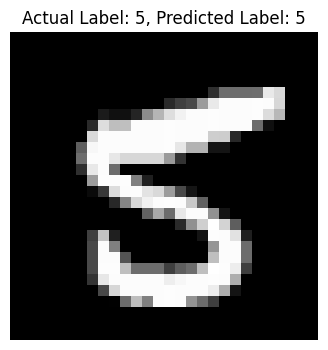
\includegraphics[width=3.5cm]{Lab-2/data/5.png}
\caption{Image generated for label 5.}
\label{fig:sample}
\end{figure}

\FloatBarrier

\begin{figure}[ht]
\centering
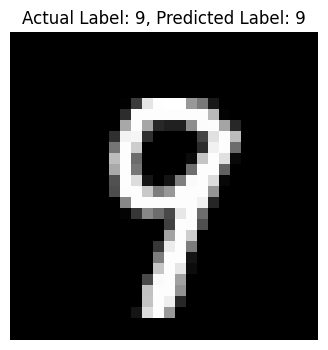
\includegraphics[width=3.5cm]{Lab-2/data/9.png}
\caption{Image sample generated for label 9.}
\label{fig:sample}
\end{figure}

\FloatBarrier

\begin{figure}[ht]
\centering
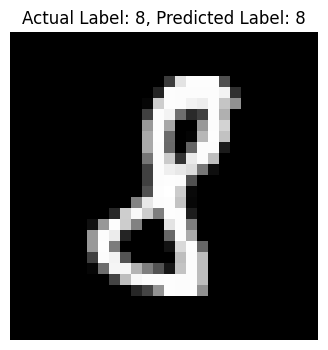
\includegraphics[width=3.5cm]{Lab-2/data/8.png}
\caption{Image sample generated for label 8.}
\label{fig:sample}
\end{figure}

\FloatBarrier

\begin{figure}[ht]
\centering
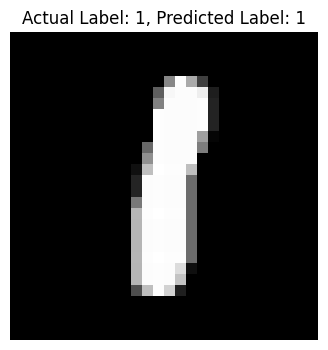
\includegraphics[width=3.5cm]{Lab-2/data/1.png}
\caption{Image sample generated for label 1.}
\label{fig:sample}
\end{figure}

\FloatBarrier

\section{Problem-3(a)}
Find out a few samples where the predicted label is incorrect.\\

\textbf{Solution 3(a): }
\lstinputlisting[style=mystyle]{Lab-2/MNIST_3.py}\\

\textbf{Output 3(a): }

\begin{figure}[ht]
\centering
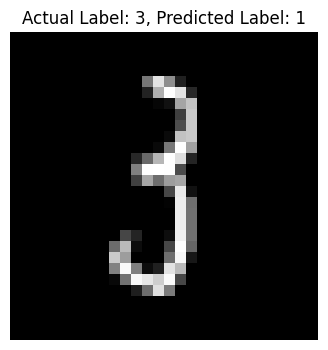
\includegraphics[width=3.5cm]{Lab-2/data/3_1.png}
\caption{Mismatched Image sample of actual label 3 with predicted label 1.}
\label{fig:sample}
\end{figure}

\FloatBarrier

\begin{figure}[ht]
\centering
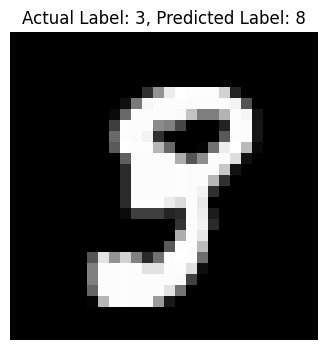
\includegraphics[width=3.5cm]{Lab-2/data/3_9.png}
\caption{Mismatched Image sample of actual label 3 with predicted label 8.}
\label{fig:sample}
\end{figure}

\FloatBarrier

\begin{figure}[ht]
\centering
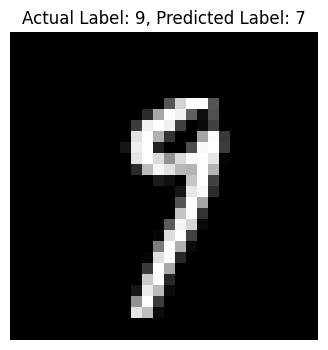
\includegraphics[width=3.5cm]{Lab-2/data/9_7.png}
\caption{Mismatched Image sample of actual label 9 with predicted label 7.}
\label{fig:sample}
\end{figure}

\FloatBarrier

\section{Objective}
The second problem is on the (Apple vs Orange) classification. You are given a K-NN code for Apple vs Orange problem. Please read and understand the code. Now perform the following tasks:

\section{Problem-1(b)}
Synthetically increase the dataset size to 50 samples.\\\\

\textbf{Solution 1(b): }
\lstinputlisting[style=mystyle]{Lab-2/KNN_1.py}\\

\textbf{Output 1(b): }
\lstinputlisting[style=mystyle]{Lab-2/KNN_sol_1.txt}\\

\lstinputlisting[style=mystyle]{Lab-2/KNN_5.py}
\lstinputlisting[style=mystyle]{Lab-2/KNN_sol_7.txt}

\section{Problem-2(b)}
Edit the code so that random 80 percentage, 10 percentage, and 10 percentage samples are used for training, testing, and validation respectively.\\

\textbf{Solution 2(b): }
\lstinputlisting[style=mystyle]{Lab-2/KNN_2.py}\\

\textbf{Output 2(b): }
\lstinputlisting[style=mystyle]{Lab-2/KNN_sol_2.txt}\\

\section{Problem-3(b)}
Change the value of K to 3, 5, and 7 and compare the validation set and test set results.

\textbf{Solution 3(b): }
\lstinputlisting[style=mystyle]{Lab-2/KNN_3.py}\\

\textbf{Output 3(b): }
\lstinputlisting[style=mystyle]{Lab-2/KNN_sol_3.txt}\\

\section{Problem-4(b)}
Write a code that draws confusion matrices for different K.

\textbf{Solution 4(b): }
\lstinputlisting[style=mystyle]{Lab-2/KNN_4.py}\\

\textbf{Output 4(b): }
\lstinputlisting[style=mystyle]{Lab-2/KNN_sol_4.txt}\\

\begin{figure}[ht]
\centering
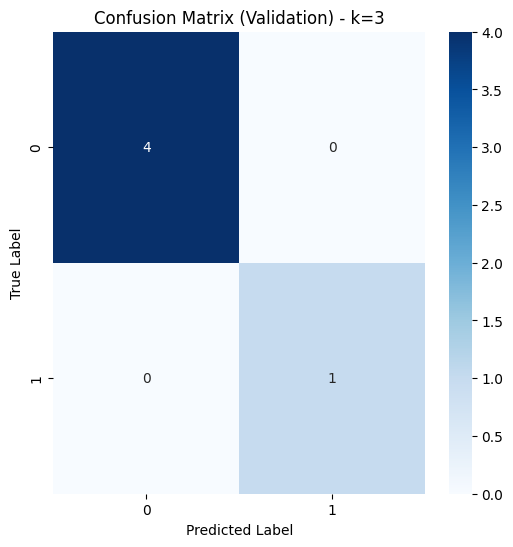
\includegraphics[width=5.7cm]{Lab-2/data/k_3.png}
\caption{Confusion Matrix ( Validation ) for k=3.}
\label{fig:sample}
\end{figure}

\FloatBarrier

\lstinputlisting[style=mystyle]{Lab-2/KNN_sol_5.txt}\\

\begin{figure}[ht]
\centering
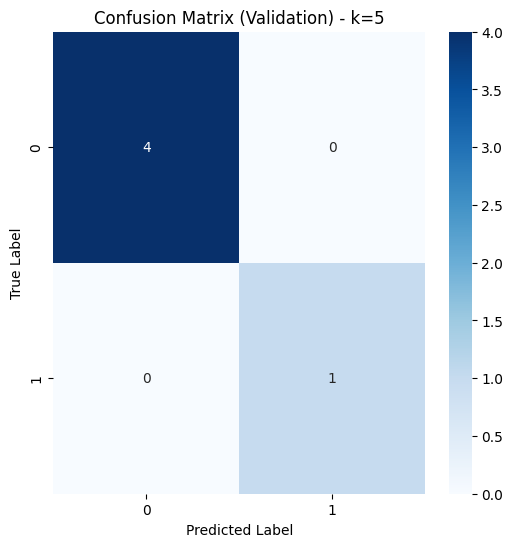
\includegraphics[width=5.7cm]{Lab-2/data/k_5.png}
\caption{Confusion Matrix ( Validation ) for k=5.}
\label{fig:sample}
\end{figure}

\FloatBarrier

\lstinputlisting[style=mystyle]{Lab-2/KNN_sol_6.txt}
\begin{figure}[ht!]
\centering
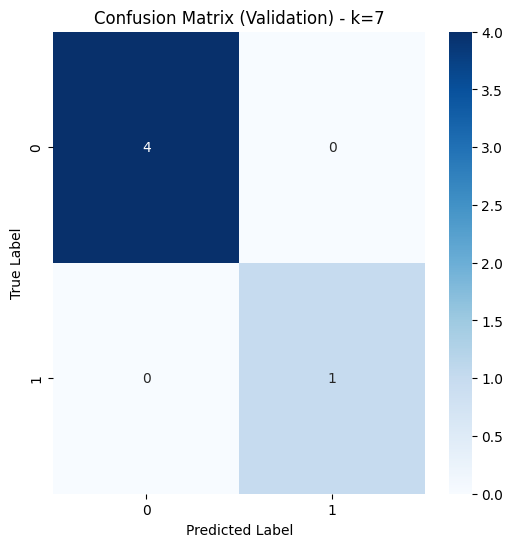
\includegraphics[width=5.7cm]{Lab-2/data/k_7.png}
\caption{Confusion Matrix ( Validation ) for k=7.}
\label{fig:sample}
\end{figure}
